\section{Backend}

The backend can be given a walk through using OpenAPI which is a specification for machine readable interfaces, producing and consuming restful API services. 

\subsection{OpenAPI}
The OpenAPI documentation is accessible through the backend server. There are separations based on each component in the LMS.

\subsubsection{Purpose}
The purpose of the OpenAPI specification is to show a list of endpoints for each component including inputs and output responses.

\subsubsection{What Was Implemented}
A user with access to the OpenAPI document can view specific endpoints through their sections. 

\begin{figure}[h!]
    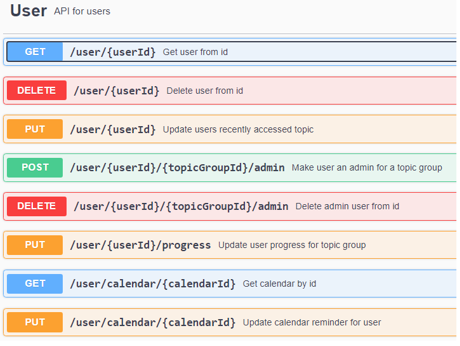
\includegraphics[scale=1]{backend_walkthrough_sample_endpoints}
    \centering
    \caption{OpenAPI endpoints}
\end{figure}

The user can click on any endpoint and then view the required inputs and sample outputs of the endpoint. Then once the user has clicked on an endpoint, they are able to enter parameters to get a response tailored to their inputs.

\begin{figure}[h!]
    \centering
    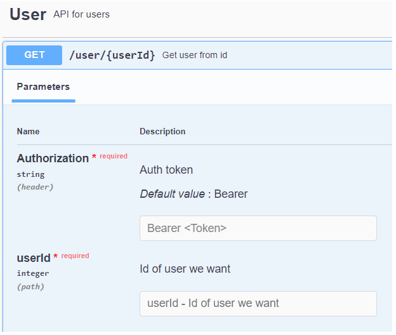
\includegraphics[scale=1]{backend_walkthrough_endpoint_params}
    \caption{Endpoint Parameters}
\end{figure}

\begin{figure}[h!]
    \centering
    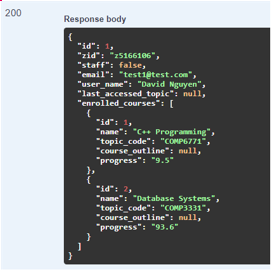
\includegraphics[scale=1]{backend_walkthrough_response}
    \caption{Output of endpoint}
\end{figure}

\subsubsection{How It Was Implemented}
This component was implemented using OpenAPI specification, which is a specification for visualising RESTful webservices. The APIs are created using NodeJS and Express and then visualised in the OpenAPI specification, and the backend handles the input parameters given through OpenAPI. Additionally, when the user clicks the execute button the request is sent to the backend and then the output response can be viewed in the relevant endpoint in OpenAPI.

\subsubsection{Considerations}
Instead of having a single list of endpoints, the endpoints were separated based on the project features. This allows users to quickly identify their desired endpoint and sections. 